The analysis uses two methods of estimating the contribution of background processes (i.e., those other than \ttH).
The first estimates the background directly from data by fitting events in the \mgg sidebands, defined as $\mgg \in [100, 115] \cup [135, 180]$ GeV, by fitting a variety of functional forms.
The second estimates the background from individual descriptions of each background process.
These descriptions are taken primarily from simulations of each process; however, data-driven descriptions of some processes are also utilized: the multi-jet and \gjets backgrounds are described with a sample of events in data from the low photon ID sideband (described in Sec.~\ref{sec:tth_datadriven}).
The first method is referred to as the ``discrete profiling method'', while the second is referred to as the ``MC description'' of the background.

The discrete profiling method is used to estimate the background in the final statistical analysis and is described in Sec.~\ref{sec:sig_bkg_models}.
The MC description of the background is used only in designing and optimizing the cuts on the BDT-bkg algorithms and is described in this section.

\subsection{Challenges of MC Description} \label{sec:tth_mc_description}
The events entering the hadronic or leptonic preselection are dominated by Standard Model processes other than \ttH.
Precise knowledge of exactly which processes enter the preselection and their relative contributions to the overall background is not strictly necessary, as the background is modeled from events in data (described in Sec.~\ref{sec:sig_bkg_models}) when performing the measurement of $\mu_{\ttH}$.
However, the BDT-bkg algorithms are designed to distinguish between \ttH and the SM background processes; to this end, an accurate description of the background is desirable.
Note that events in data cannot be used to both model the background in the measurement of $\mu_{\ttH}$ and in training the BDT-bkg algorithm, as this would bias the measurement.
The starting point for the background description used in training the BDT-bkg algorithms is simulation of the relevant SM processes.
In the hadronic channel, the dominant backgrounds at preselection level are the multi-jet, \gjets, and \dipho processes; those same processes, as well as \ttbar, \ttg, \ttgg, and \Vgamma dominate for the leptonic channel.
The \mgg distribution for events in data and simulation are shown in Fig.~\ref{fig:tth_mgg_presel_datamc}.
The exact yields and relative contributions of all considered background processes are shown in Table~\ref{tab:tth_presel_datamc}.

\begin{figure} [h!]
    \centering
    \begin{tabular}{c c}
        \includegraphics[width=0.48\linewidth,page=1]{{figures/tth/ttHHadronic_RunII_MVA_Presel_v4.11_9Jun2020_no_scale_histogramsRunIIstd_linear}.pdf} &
        \includegraphics[width=0.48\linewidth,page=1]{{figures/tth/ttHLeptonic_RunII_MVA_Presel_v4.11_9Jun2020_histogramsRunIIstd_linear}.pdf} 
    \end{tabular}
    \caption{Diphoton invariant mass distributions for events from data and simulation entering the hadronic (right) and leptonic (left) channel preselections. Events in data are blinded in the region $\mgg \in [120, 130]$.}
    \label{fig:tth_mgg_presel_datamc}
\end{figure}

\begin{table} [h!]
    \centering
    \begin{tabular}{c c}
    	\begin{tabular}{ r || r | r} \hline \hline
			Process & Yield & $\mathcal F$ of bkg \\ \hline
			\dipho & 40972.68 $\pm$ 75.87 & 0.32 \\ 
			\gjets & 52434.13 $\pm$ 1960.51 & 0.41 \\ 
			Multi-jet & 29277.57 $\pm$ 3566.18 & 0.23 \\ 
			\ttgg & 642.31 $\pm$ 35.09 & 0.01 \\ 
			\ttg & 1538.53 $\pm$ 68.77 & 0.01 \\ 
			\ttb & 997.19 $\pm$ 74.15 & 0.01 \\ 
			Drell-Yan & 265.24 $\pm$ 47.48 & 0.00 \\ 
			$\text{t} + \gamma$ & 170.79 $\pm$ 26.66 & 0.00 \\ 
			V + $\gamma$ & 1237.50 $\pm$ 39.10 & 0.01 \\ 
			\ttW & 3.13 $\pm$ 0.17 & 0.00 \\ 
			\ttZ & 3.41 $\pm$ 0.15 & 0.00 \\ 
			VV & 55.06 $\pm$ 4.49 & 0.00 \\ 
			tV & 135.61 $\pm$ 7.57 & 0.00 \\  \hline
			tHq & 5.53 $\pm$ 0.00 & 0.00 \\
            tHW & 1.44 $\pm$ 0.00 & 0.00 \\
			ggH & 199.20 $\pm$ 1.80 & 0.00 \\
            VH & 22.94 $\pm$ 0.22 & 0.00 \\
            VBF & 18.78 $\pm$ 0.24 & 0.00 \\ 
            All bkg. & 128029.09 $\pm$ 4072.22 & 1.00 \\ \hline 
            Data & 233060.00 $\pm$ 482.76 & 1.82 \\ \hline 
			\ttH & 48.03 $\pm$ 0.32 & 0.00 \\  \hline \hline
		\end{tabular}    
		&
		\begin{tabular}{ r || r | r} \hline \hline
			Process & Yield & $\mathcal F$ of bkg \\ \hline
            \dipho & 1067.40 $\pm$ 13.85 & 0.15 \\ 
			\gjets & 1070.57 $\pm$ 236.09 & 0.15 \\ 
			Multi-jet & 482.43 $\pm$ 343.91 & 0.07 \\ 
			\ttgg & 313.58 $\pm$ 8.39 & 0.04 \\ 
			\ttg & 542.93 $\pm$ 11.70 & 0.08 \\ 
			\ttb + Jets & 159.21 $\pm$ 6.15 & 0.02 \\ 
			Drell-Yan & 220.56 $\pm$ 39.78 & 0.03 \\ 
            $\text{t} + \gamma$ & 37.43 $\pm$ 13.28 & 0.01 \\ 
			V + $\gamma$ & 3081.67 $\pm$ 56.46 & 0.43 \\ 
			\ttW & 3.61 $\pm$ 0.18 & 0.00 \\ 
			\ttZ & 4.75 $\pm$ 0.17 & 0.00 \\ 
			VV & 51.79 $\pm$ 4.12 & 0.01 \\ 
			tV & 61.17 $\pm$ 4.88 & 0.01 \\  \hline
			tHq & 1.83 $\pm$ 0.00 & 0.00 \\ 
            tHW & 0.79 $\pm$ 0.00 & 0.00 \\ 
			ggH & 4.90 $\pm$ 0.25 & 0.00 \\ 
            VH & 10.67 $\pm$ 0.14 & 0.00 \\ 
            VBF & 0.74 $\pm$ 0.04 & 0.00 \\ \hline 
			All bkg. & 7138.36 $\pm$ 423.60 & 1.00 \\ \hline
			Data & 9450.00 $\pm$ 97.21 & 1.32 \\ \hline
			\ttH & 22.36 $\pm$ 0.21 & 0.00 \\  \hline \hline
		\end{tabular}
    \end{tabular}
    \caption{Yields and fraction of total background by process for the hadronic (left) and leptonic (right) channel preselections. Backgrounds not explicitly shown in Fig.~\ref{fig:tth_mgg_presel_datamc} are consolidated in the ``Other'' category.}
	\label{tab:tth_presel_datamc}
\end{table}

In both channels, the overall yield from the background description given by simulation is somewhat smaller than what is observed in data.
This underprediction can be primarily attributed to a poor MC description of the multi-jet and \gjets processes, as the following section illustrates (and remedies). 

\subsection{Data-Driven Description of Multi-jet and \gjets Backgrounds} \label{sec:tth_datadriven}
To better understand the reason for the large discrepancies between data and simulation shown in Fig.~\ref{fig:tth_mgg_presel_datamc} and Table~\ref{tab:tth_presel_datamc}, it is helpful to study the discrepancy as a function of the event kinematics.
The distribution of minimum photon ID, defined as the smaller of the two photon ID BDT scores in the event, illustrates that the underprediction from simulation stems primarily from low values of minimum photon ID, as shown in Fig.~\ref{fig:tth_phoID_presel_datamc}.
\begin{figure} [h!]
    \centering
    \begin{tabular}{c c}
        \includegraphics[width=0.48\linewidth,page=42]{{figures/tth/ttHHadronic_RunII_MVA_Presel_v4.11_9Jun2020_no_scale_histogramsRunIIstd_linear}.pdf} &
        \includegraphics[width=0.48\linewidth,page=43]{{figures/tth/ttHLeptonic_RunII_MVA_Presel_v4.11_9Jun2020_histogramsRunIIstd_linear}.pdf}
    \end{tabular}
    \caption{Minimum photon ID distributions for events from data and simulation entering the hadronic (right) and leptonic (left) channel preselections. Events in data are blinded in the region $\mgg \in [120, 130]$.}
    \label{fig:tth_phoID_presel_datamc}
\end{figure}

The underprediction from simulation is especially pronounced at lower values of minimum photon ID, while the agreement becomes better for higher values. 
As the photon ID BDT discriminates between prompt and fake photons, we expect the lower end of the distribution to have a larger contribution from fake photons.
Thus, Fig.~\ref{fig:tth_phoID_presel_datamc} suggests that simulation provides an inadequate description of events with at least one fake photon. 

To improve the description of events with at least one fake photon (i.e. multi-jet and \gjets events), a sample of events from an orthogonal region of data is used in place of the simulation when training BDT-bkg.
This region, the ``low photon ID sideband'', is defined identically to the preselection except for the cut on minimum photon ID: the preselection requires minimum photon ID $>-0.7$, while the low photon ID sideband requires $-0.9<$ minimum photon ID $<-0.7$.
The preselection and low photon ID sideband are depicted in Fig.~\ref{fig:tth_low_photon_ID_sideband_pic}. 
\begin{figure} [h!]
    \centering
    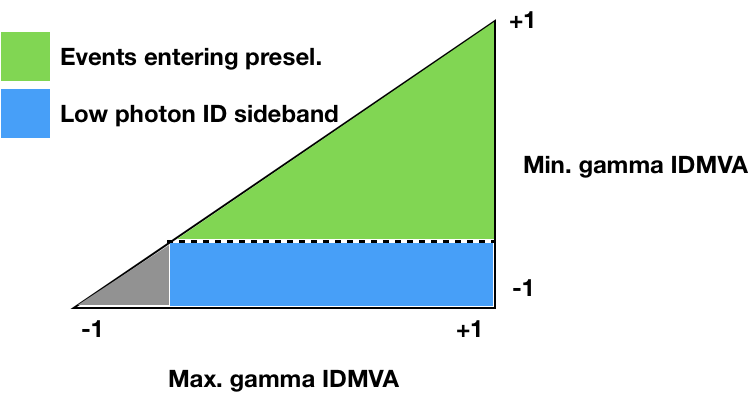
\includegraphics[width=0.75\linewidth]{{figures/tth/low_photon_ID_sideband.png}}
    \caption{Depiction of the relationship between preselection (green) and low photon ID sideband (blue).}
    \label{fig:tth_low_photon_ID_sideband_pic}
\end{figure}
Replacing the MC description of multi-jet and \gjets with the data-driven description relies on the assumption that events in the low photon ID sideband are exlusively multi-jet and \gjets events.
Simulation indicates that $> 95\%$ of events in the low photon ID sideband are multi-jet or \gjets events.

An immediate challenge in making the replacement of MC description of multi-jet and \gjets $\to$ data-driven description of multi-jet and \gjets is the fact that the minimum photon ID for these events and the minimum photon ID for events in the preselection are disjoint, by definition.
This is problematic because of the fact that minimum photon ID is used as a training feature for the BDT-bkg algorithms.
Training with an unaltered minimum photon ID distribution would lead the BDT to eliminate all of these background events with a single cut at the value of minimum photon ID that defines the sideband.
To make the data-driven sample feasible for use in training the BDT-bkg algorithm, its minimum photon ID distribution should be altered such that it resembles the expected distribution of multi-jet and \gjets events in the preselection region.

To generate the proper minimum photon ID distribution for events in the data-driven sample, the minimum photon ID score of each event is replaced by a randomly drawn value from a probability distribution function that describes the expected distribution of multi-jet and \gjets in the preselection.
The procedure is simplified by assuming that for events in the low photon ID sideband the photon with the lower photon ID score is always a fake photon.
This assumption is always true for multi-jet events (which have two fake photons), and from simulation, is found to be true for $> 95\%$ of \gjets events.
Under this assumption, the expected distribution of minimum photon ID for multi-jet and \gjets events in the preselection region can be approximated by the probability distribution function of photon ID for fake photons, called the ``fake pdf''.
The fake pdf is derived from simulation using the photon ID distribution of photons which are identified as fakes at generator-level.
For ease of drawing random values from this pdf, a histogram of the fake pdf is fitted with a seventh-order polynomial, shown in Fig.~\ref{fig:tth_fake_pdf}.
\begin{figure} [h!]
    \centering
    \includegraphics[width=0.75\linewidth]{{figures/tth/fake_photonID_shape.pdf}}
    \caption{Histogram of photon ID for fake photons in simulation (blue) and resulting seventh-order polynomial.}
    \label{fig:tth_fake_pdf}
\end{figure}
However, as minimum and maximum photon ID are strongly correlated by construction, the maximum photon ID distribution for events from the low photon ID sideband will also be different than the maximum photon ID distribution for events from the preselection.
In general, events from the low photon ID sideband will have lower maximum photon ID scores than events from the preselection.
To address the differences in maximum photon ID, an additional weight is applied to each event to correct for the fact that the distribution is biased towards lower values of maximum photon ID:
\begin{align} \label{eqn:impute_weight}
    w &= \frac{\int_{B}^{\text{max } \gamma \text{ ID}} \text{fake pdf}}{\int_{A}^{B} \text{fake pdf}} \\
    A &\equiv \text{minimum value of photon ID in the low photon ID sideband} = -0.9 \\
    B &\equiv \text{preselection cut value on minimum photon ID} = -0.7
\end{align} 
Qualitatively, the term of the numerator of Eqn.~\ref{eqn:impute_weight} increases the contribution of events from the low photon ID sideband with high values of maximum photon ID.
The term in the denominator is simply an overall normalization factor.
After applying the per-event weight, the overall normalization of the data-driven sample is determined with a simultaneous fit to data of the minimum and maximum photon ID distributions in the preselection.
The normalization of \dipho is also allowed to float in this fit, while the normalization of all other background processes are taken to be fixed.
\begin{figure} [htbp!]
    \centering
    \begin{tabular}{c c}
        \includegraphics[width=0.48\linewidth,page=42]{{figures/tth/ttHHadronic_RunII_MVA_Presel_v4.11_9Jun2020_impute_no_scale_histogramsRunIIstd_linear}.pdf} &
        \includegraphics[width=0.48\linewidth,page=43]{{figures/tth/ttHHadronic_RunII_MVA_Presel_v4.11_9Jun2020_impute_no_scale_histogramsRunIIstd_linear}.pdf} \\
		\includegraphics[width=0.48\linewidth,page=42]{{figures/tth/ttHHadronic_RunII_MVA_Presel_v4.11_9Jun2020_impute_histogramsRunIIstd_linear}.pdf} &
        \includegraphics[width=0.48\linewidth,page=43]{{figures/tth/ttHHadronic_RunII_MVA_Presel_v4.11_9Jun2020_impute_histogramsRunIIstd_linear}.pdf} \\
    \end{tabular}
    \caption{Distributions of minimum (left) and maximum (right) photon ID in the hadronic preselection before (top) and after (bottom) fitting the normalization of the data-driven description of multi-jet and \gjets and the MC description of \dipho.}
    \label{fig:tth_phoID_fits}
\end{figure}

\begin{table} [h]
	\centering
	\begin{tabular}{|l|| r| r| r|} \hline
		Template & Initial Fraction & Fitted Fraction & Scale \\ \hline
		$ \gamma $ + jets (fake/prompt) & 0.68 & 0.73 $ \pm $ 0.00 & 1.07 \\
		$ \gamma \gamma $ + jets (prompt/prompt) & 0.18 & 0.25 $ \pm $ 0.00 & 1.42 \\ \hline
	\end{tabular}
	\caption{Results of binned fit of diphoton templates in the hadronic preselection, with template for prompt/prompt taken from MC simulation and template for fake/fake and fake/prompt taken from the data-driven description.}
    \label{tab:tth_phoID_fits}
\end{table}
The minimum and maximum photon ID distributions are shown pre-/post-fit in Fig.~\ref{fig:tth_phoID_fits} and the results of the fit are shown in Table~\ref{tab:tth_phoID_fits}.
The agreement with data is significantly improved when using the data-driven description of multi-jet and \gjets in place of the MC description, as can be seen by comparing Fig.~\ref{fig:tth_phoID_presel_datamc} and Fig.~\ref{fig:tth_phoID_fits}.
This improvement is consistently seen in other distributions as well, including the jet and b-jet multiplicities shown in Fig.~\ref{fig:tth_impute_compare}.
\begin{figure} [htbp!]
    \centering
    \begin{tabular}{c c}
        \includegraphics[width=0.48\linewidth,page=5]{{figures/tth/ttHHadronic_RunII_MVA_Presel_v4.11_9Jun2020_no_scale_histogramsRunIIstd}.pdf} &
        \includegraphics[width=0.48\linewidth,page=5]{{figures/tth/ttHHadronic_RunII_MVA_Presel_v4.11_9Jun2020_impute_histogramsRunIIstd}.pdf} \\
        \includegraphics[width=0.48\linewidth,page=8]{{figures/tth/ttHHadronic_RunII_MVA_Presel_v4.11_9Jun2020_no_scale_histogramsRunIIstd}.pdf} &
        \includegraphics[width=0.48\linewidth,page=8]{{figures/tth/ttHHadronic_RunII_MVA_Presel_v4.11_9Jun2020_impute_histogramsRunIIstd}.pdf} \\
    \end{tabular}
    \caption{Agreement between data and MC description of background for jet multiplicity (top) and b-jet multiplicity (bottom), shown with both the MC description of multi-jet and \gjets (left) and the data-driven description of multi-jet and \gjets (right).} 
    \label{fig:tth_impute_compare}
\end{figure}
%Using events from the low photon ID sideband to describe the multi-jet and \gjets processes relies on several assumptions:
%\begin{enumerate}
%    \item The low photon ID sideband is composed completely of multi-jet and \gjets events.
%    \item The photon with the smaller photon ID value is always a fake photon.
%    \item The output of photon ID BDT is uncorrelated with other input features used in training the BDT-bkg algorithms.
%\end{enumerate}

As the MC description of the background is used only for designing and optimizing the cuts on the BDT-bkg algorithms, the bottom-line test of the merit of the data-driven description is BDT-bkg performance.
To this end, we compare the performance of the BDT-bkg algorithm trained with the MC description of \gjets (including the MC description of multi-jet events was found to degrade performance because of the extremely few number of events from the multi-jet simulation samples) with the performance of the BDT-bkg algorithm trained with the data-driven description of multi-jet and \gjets, using $Z_A$ (defined in Sec.~\ref{sec:tth_za}) as an estimate of the expected signifiance obtained when using either BDT.
$Z_A$ is shown for each BDT as a function of the number of \ttH events in Fig.~\ref{fig:tth_imputing_za}.
The improvement obtained by replacing the MC description of \gjets with the data-driven description of multi-jet and \gjets, taken as the percentage difference between the maximum $Z_A$ values obtained with either method, is about 8\%.
\begin{figure} [h!]
    \centering
    \includegraphics[width=0.75\linewidth]{{figures/tth/za_comparison_data_imputing_vs_scale_mc_12Apr2020.pdf}}
    \caption{Expected significance ($Z_A$) shown as a function of the number of \ttH events passing a given cut on BDT-bkg for versions of BDT-bkg trained with the MC description of \gjets (black) and the data-driven description of multi-jet and \gjets (red). Shaded bands show the $\pm 1\sigma$ statistical uncertainty in $Z_A$.}
    \label{fig:tth_imputing_za}
\end{figure}
The data-driven description of multi-jet and \gjets events is not employed in the leptonic channel as it was not found to significantly improve BDT-bkg performance.
This is likely due to the combination of two factors:
\begin{enumerate}
    \item Events in the leptonic low photon ID sideband are not dominated by multi-jet and \gjets events to the same extent as in the hadronic channel; \ttbar and \ttg events play a significant role as well.
    \item The multi-jet and \gjets processes make up a smaller overall fraction of the background contribution in the leptonic preselection; there is a lower ceiling on improvements to BDT-bkg performance from improved description of these processes.
\end{enumerate}
